\section{Anexo: Gráficos adicionales}

\begin{figure}[ht]
    \centerfloat
    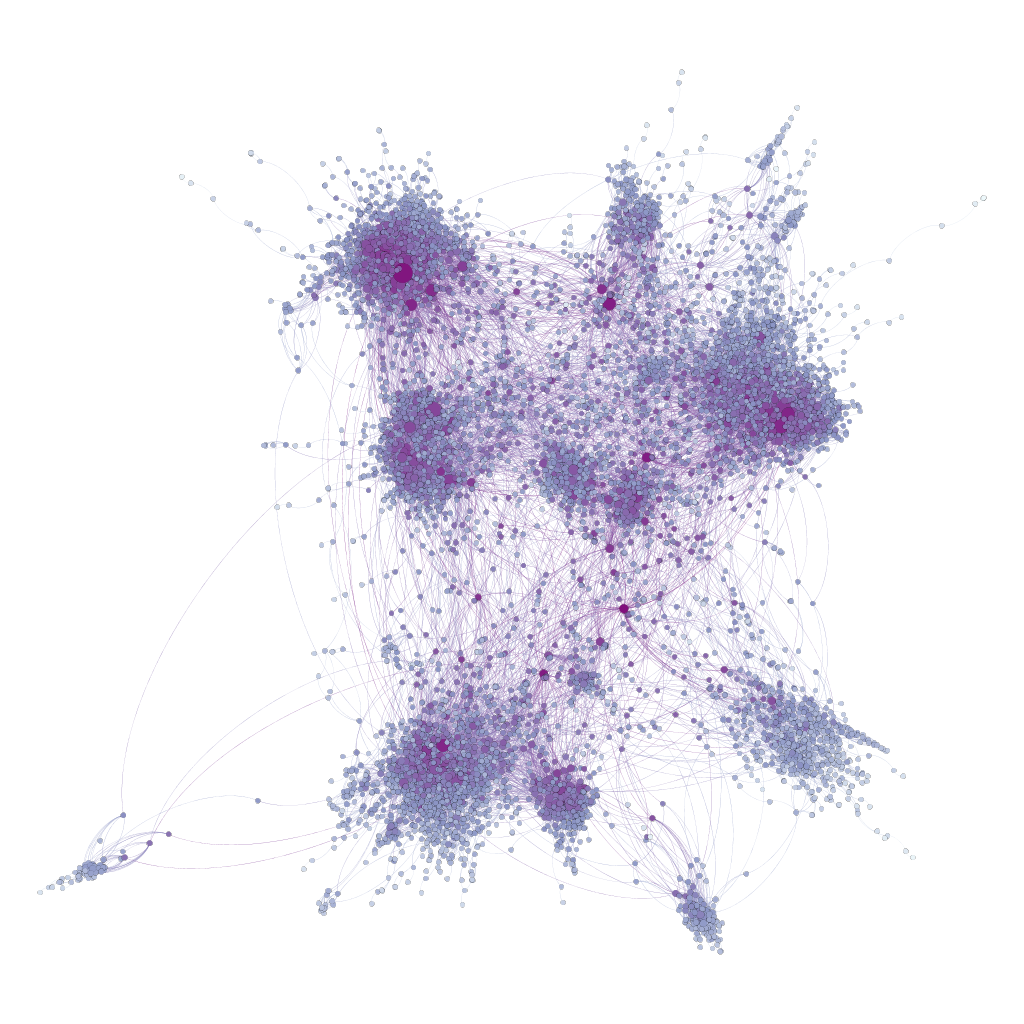
\includegraphics[width=1.095\textwidth]{img/resultados/grado-cercania.png}
    \caption{A mayor tamaño de nodo mayor grado. Mayor intensidad de violeta implica mayor cercanía.}
\end{figure}

\begin{figure}[ht]
    \centerfloat
    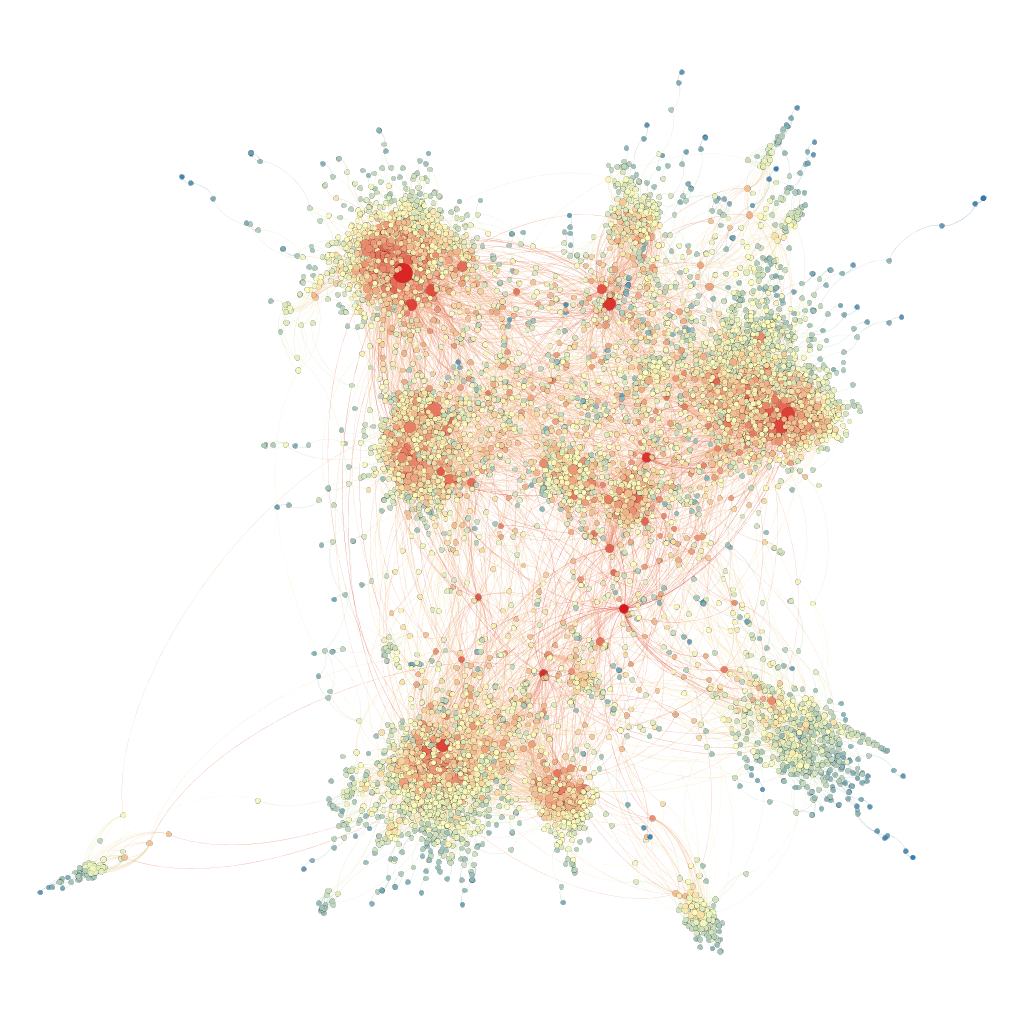
\includegraphics[width=1.3\textwidth]{img/resultados/grado-cercania2.png}
    \caption{A mayor tamaño de nodo mayor grado. Azul implica menor cercanía, rojo más.}
\end{figure}

\begin{figure}[ht]
    \centerfloat
    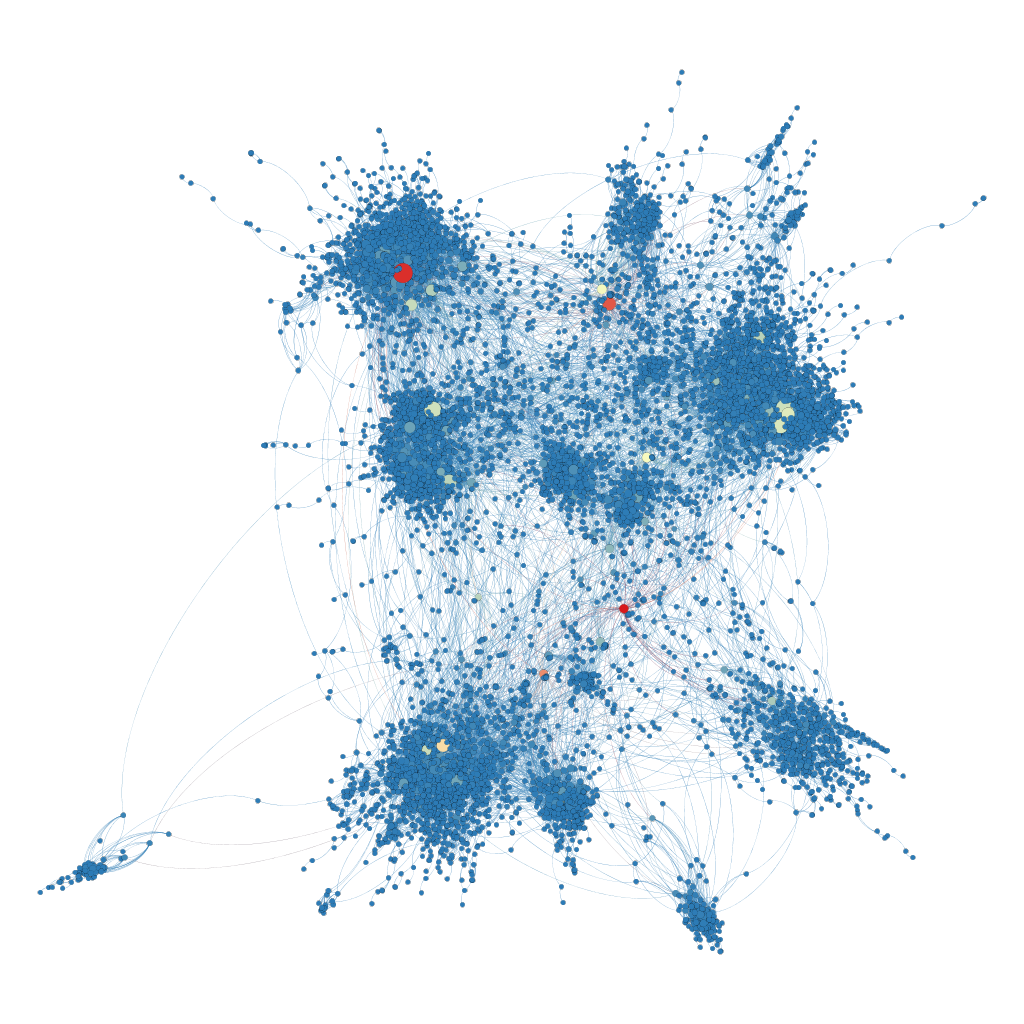
\includegraphics[width=1.3\textwidth]{img/resultados/grado-intermediacion.png}
    \caption{A mayor tamaño de nodo mayor grado. Azul implica menor intermediación, rojo más.}
\end{figure}

\begin{figure}[ht]
    \centerfloat
    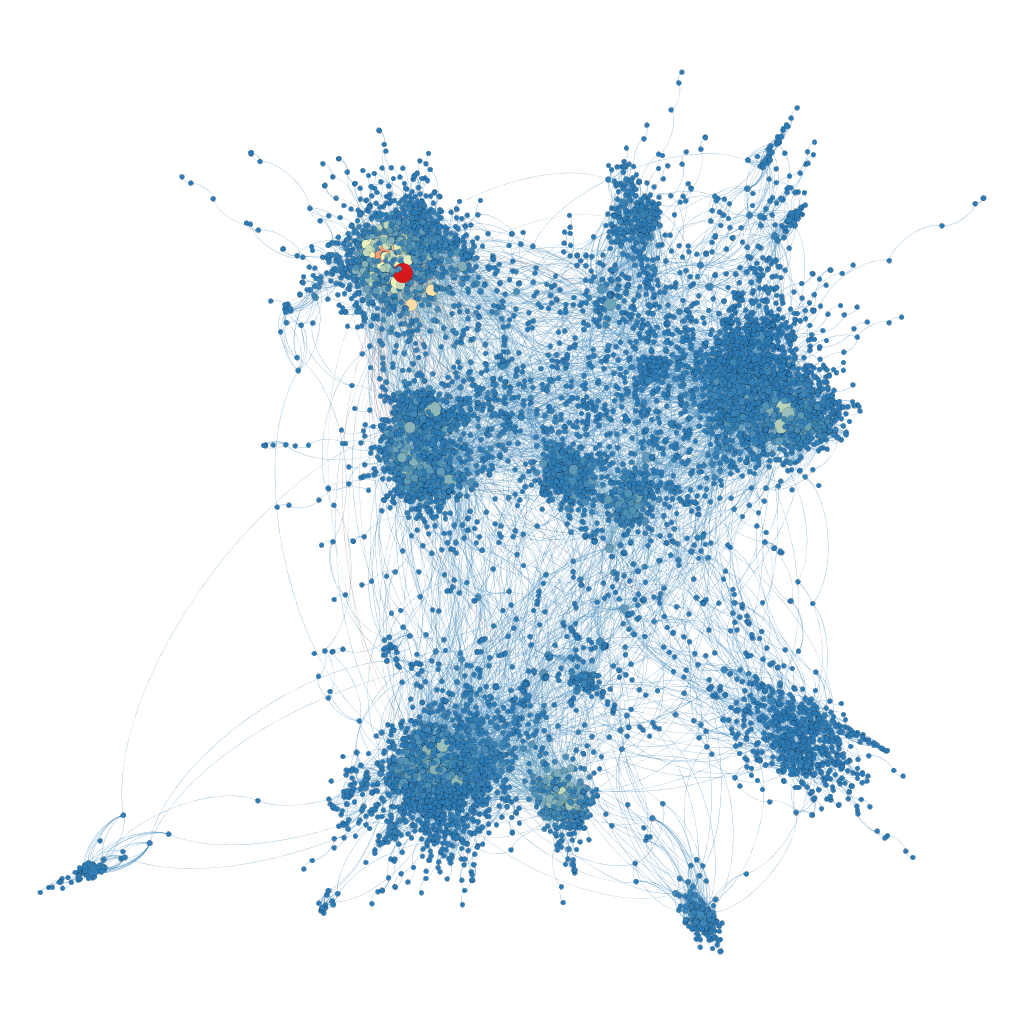
\includegraphics[width=1.3\textwidth]{img/resultados/grado-vectorPropio.png}
    \caption{A mayor tamaño de nodo mayor grado. Azul implica menor vector propio, rojo más.}
\end{figure}

\begin{figure}[ht]
    \centerfloat
    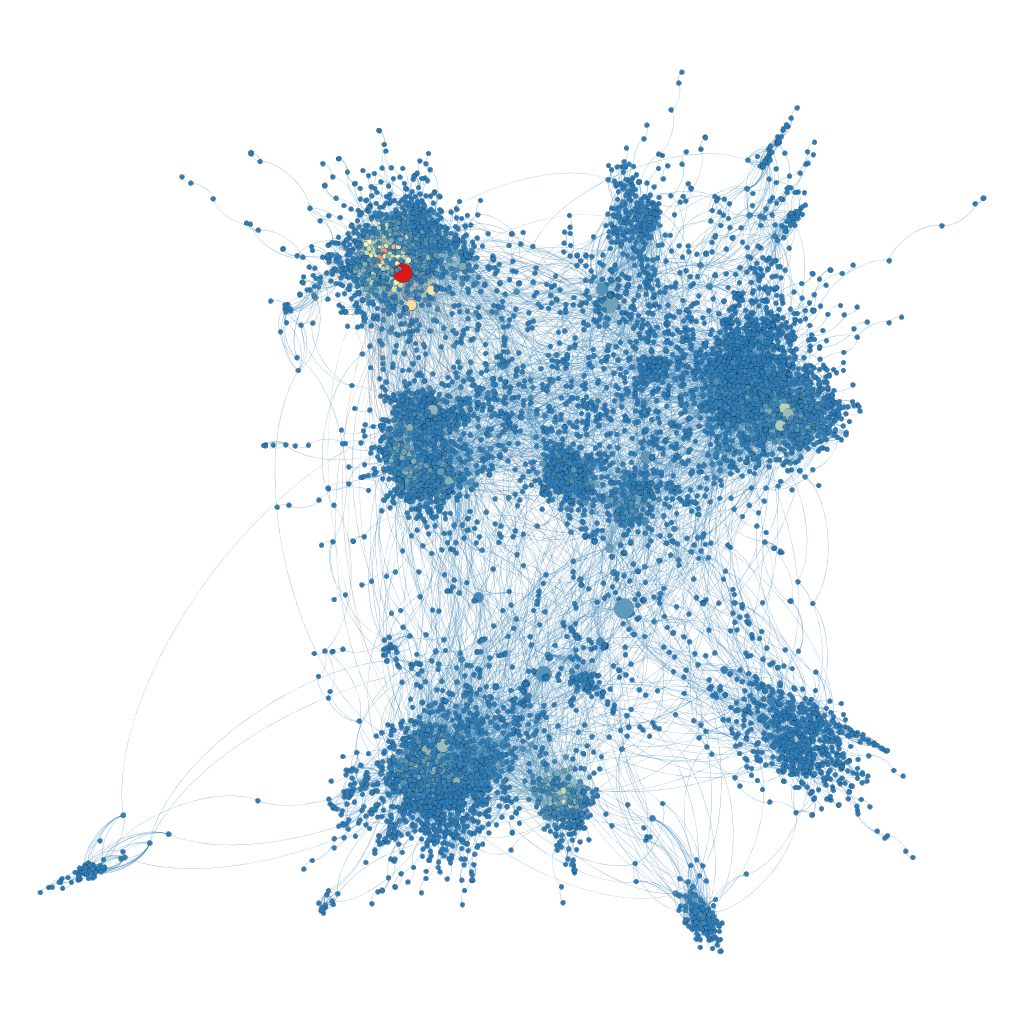
\includegraphics[width=1.3\textwidth]{img/resultados/intermediacion-vectorPropio.png}
    \caption{A mayor tamaño de nodo mayor intermediación. Azul implica menor vector propio, rojo más.}
\end{figure}